\begin{figure}[H]
    \centering


\tikzset{every picture/.style={line width=0.75pt}} %set default line width to 0.75pt        

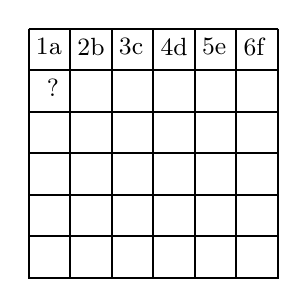
\begin{tikzpicture}[x=0.75pt,y=0.75pt,yscale=-1,xscale=1]
%uncomment if require: \path (0,300); %set diagram left start at 0, and has height of 300

%Shape: Grid [id:dp6553431843109427] 
\draw  [draw opacity=0] (139.93,60.8) -- (260.13,60.8) -- (260.13,181.47) -- (139.93,181.47) -- cycle ; \draw   (139.93,60.8) -- (139.93,181.47)(159.93,60.8) -- (159.93,181.47)(179.93,60.8) -- (179.93,181.47)(199.93,60.8) -- (199.93,181.47)(219.93,60.8) -- (219.93,181.47)(239.93,60.8) -- (239.93,181.47)(259.93,60.8) -- (259.93,181.47) ; \draw   (139.93,60.8) -- (260.13,60.8)(139.93,80.8) -- (260.13,80.8)(139.93,100.8) -- (260.13,100.8)(139.93,120.8) -- (260.13,120.8)(139.93,140.8) -- (260.13,140.8)(139.93,160.8) -- (260.13,160.8)(139.93,180.8) -- (260.13,180.8) ; \draw    ;

% Text Node
\draw (141.93,63.8) node [anchor=north west][inner sep=0.75pt]  [font=\small] [align=left] {1a};
% Text Node
\draw (144.27,83.47) node [anchor=north west][inner sep=0.75pt]  [font=\small] [align=left] {\begin{minipage}[lt]{8.67pt}\setlength\topsep{0pt}
\begin{center}
?
\end{center}

\end{minipage}};
% Text Node
\draw (241.93,63.8) node [anchor=north west][inner sep=0.75pt]  [font=\small] [align=left] {6f};
% Text Node
\draw (221.93,63.8) node [anchor=north west][inner sep=0.75pt]  [font=\small] [align=left] {5e};
% Text Node
\draw (201.93,63.8) node [anchor=north west][inner sep=0.75pt]  [font=\small] [align=left] {4d};
% Text Node
\draw (181.93,63.8) node [anchor=north west][inner sep=0.75pt]  [font=\small] [align=left] {3c};
% Text Node
\draw (161.93,63.8) node [anchor=north west][inner sep=0.75pt]  [font=\small] [align=left] {2b};


\end{tikzpicture}
    
\end{figure}